\documentclass[tikz]{standalone}


\usepackage{xcolor}
% \usepackage[inline,shortlabels]{enumitem}

\usepackage{tikz}
\usetikzlibrary{chains, shapes, arrows, calc} %, calc, fit}

\newcommand{\red}[1]{{\color{red} #1}}
\def\todo{\red{TODO}}

\begin{document}

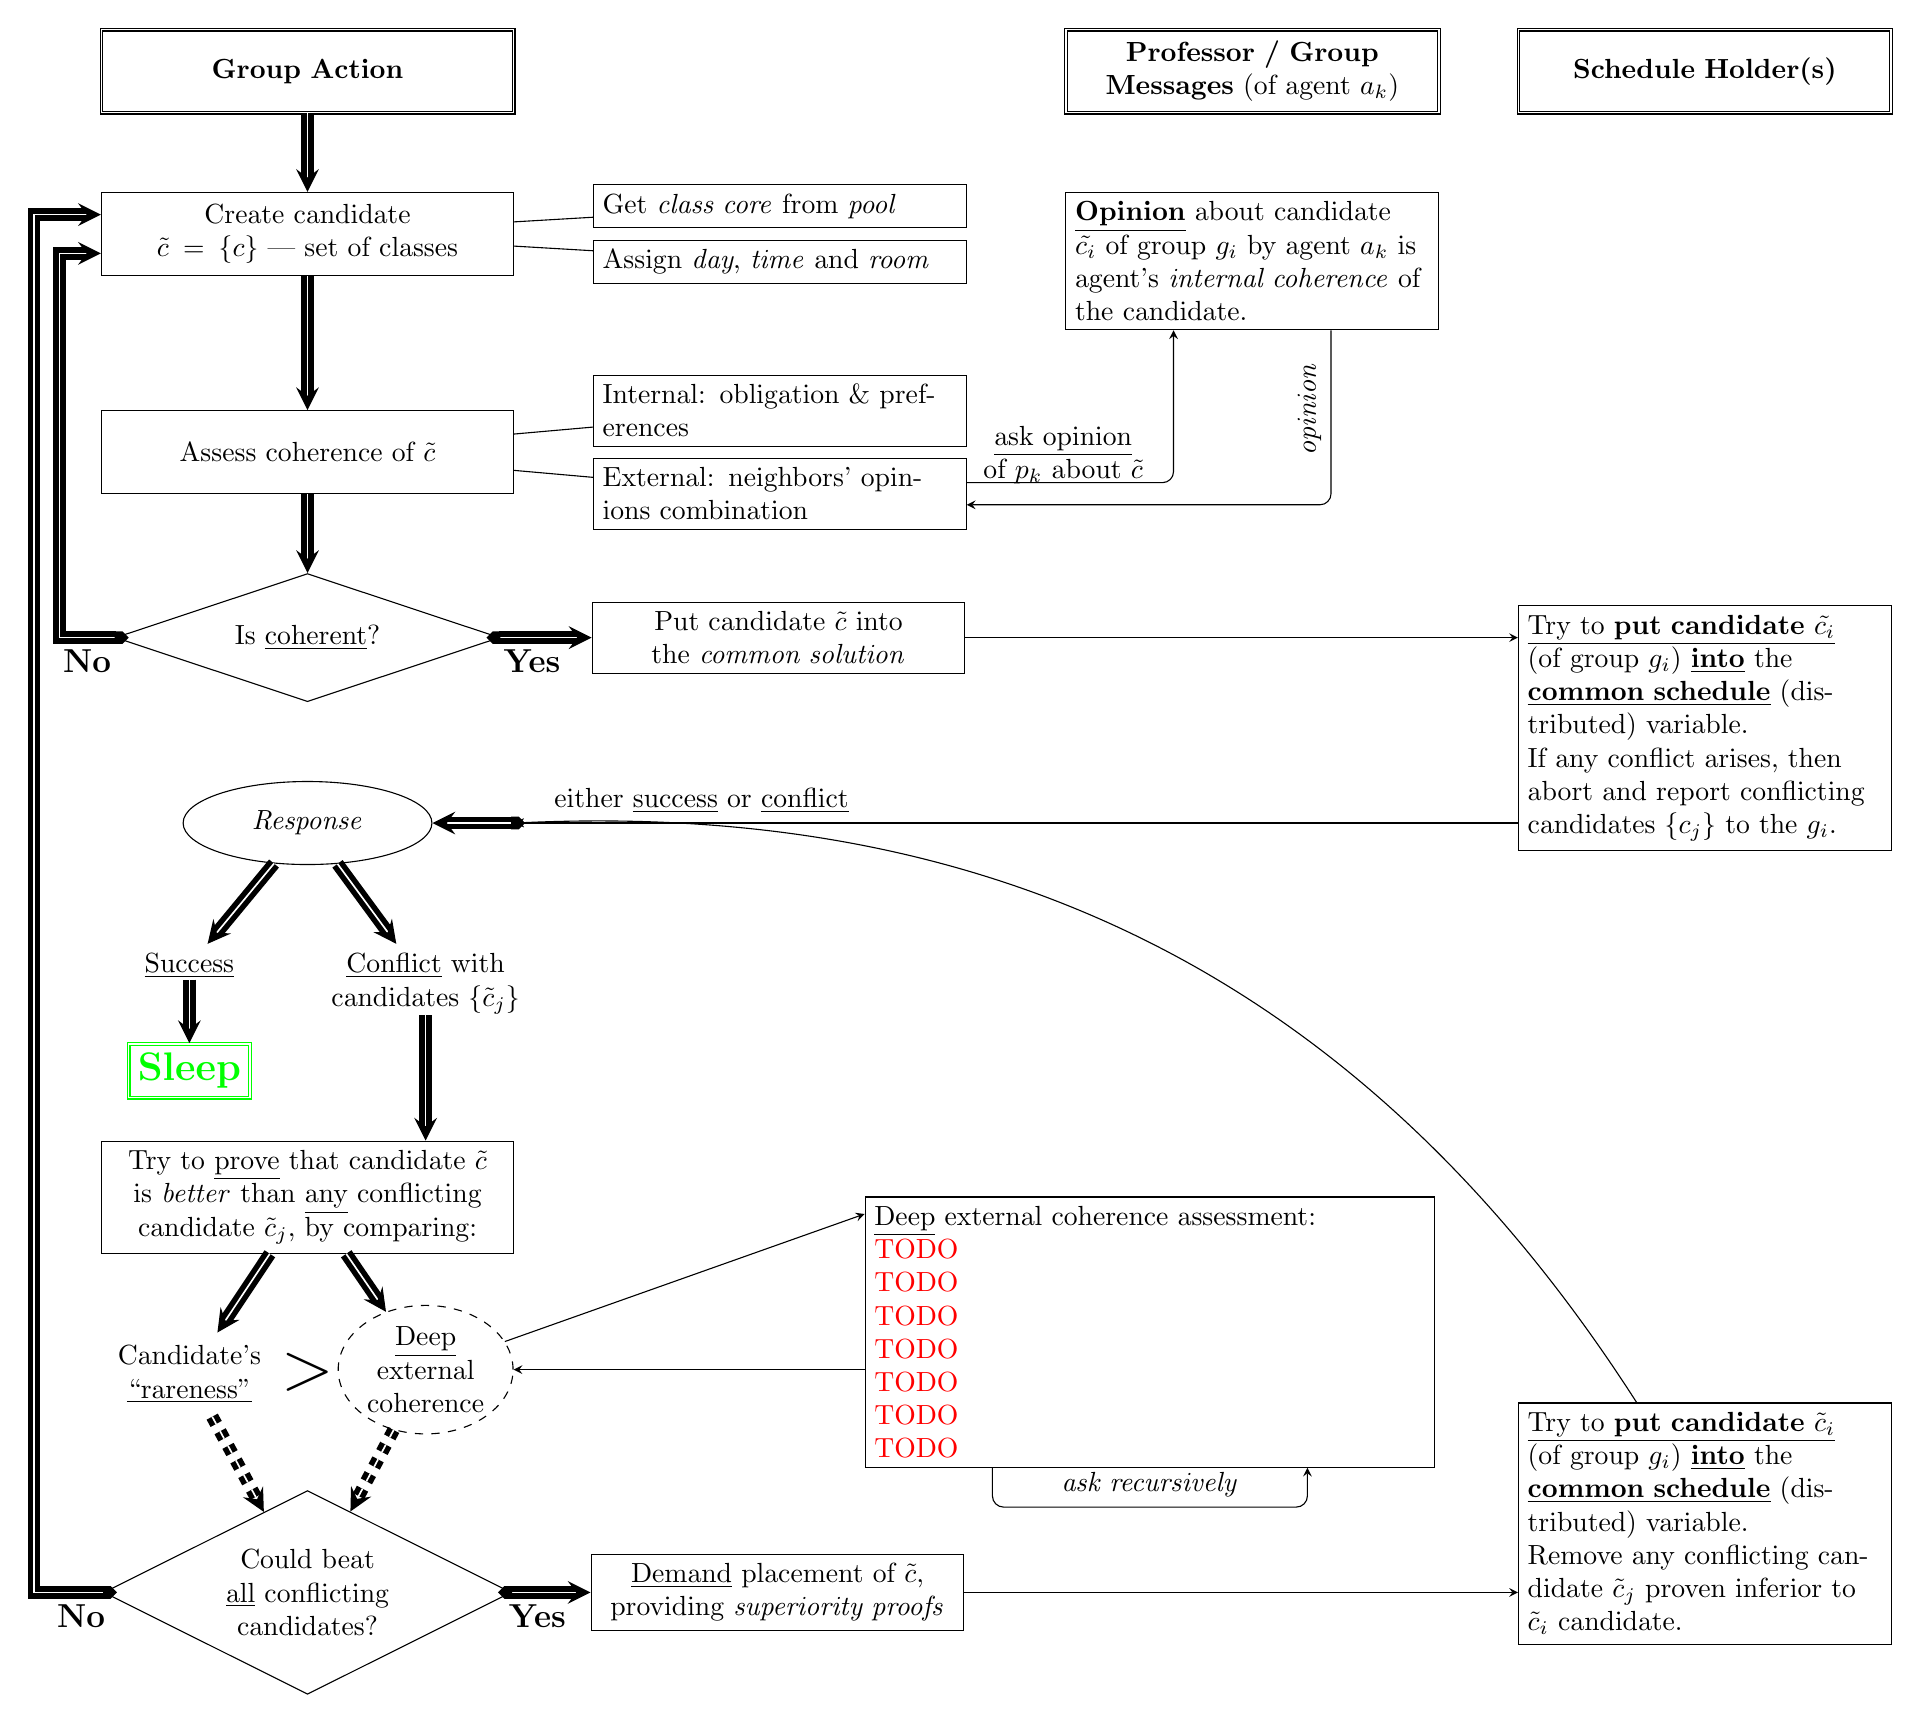
\begin{tikzpicture}[
  start chain=0 going below,
  gact/.style={on chain=0, text width=5cm, minimum height=30pt, align=center},
  start chain=1 going below,
  amsg/.style={on chain=1, text width=4.5cm, minimum height=30pt},
  start chain=2 going below,
  holder/.style={on chain=2, text width=4.5cm, minimum height=30pt},
  gact_if/.style={gact, draw, diamond, shape aspect=3, text width=3cm},
  extracol/.style={text width=4.5cm},
  % mymark/.style={draw, circle, double, thick, inner sep=2pt},
  % goto/.style={draw, circle, double, dotted, inner sep=2pt},
  arr/.style={->, >=stealth},
  flow/.style={arr, double, line width=2pt},
  flow2/.style={flow, triangle 90 cap->, shorten <=-5pt},
  msg/.style={arr, sloped, rounded corners},
  center/.style={align=center}
  ]

% % % % % % % % % % % % % % % % % % % % % % % % % % % % % % % % % % % % % % % %
% Group ACT
\begin{scope}

\node[gact, draw, double] (G-Act-label) {\textbf{Group Action}};


\def\rshift{10pt}
\node[gact, draw] (G-create-c) {Create candidate $\tilde{c}=\{c\}$ --- set of classes};
% \node[mymark, left=20pt of G-create-c, yshift=30pt] (mark-Beta) {\Large $\beta$};
\node[right=of G-create-c, yshift=\rshift, draw, extracol] (G-create-cc)
    {Get \emph{class core} from \emph{pool}};
\node[right=of G-create-c, yshift=-\rshift, draw, extracol] (G-create-DTR)
    {Assign \emph{day}, \emph{time} and \emph{room}};
\draw (G-create-c) -- (G-create-cc);
\draw (G-create-c) -- (G-create-DTR);


\def\rshift{15pt}
\node[gact, draw, yshift=-20pt] (G-assess) {Assess coherence of $\tilde{c}$};
\node[right=of G-assess, yshift=\rshift, draw, extracol] (G-assess-i)
    {Internal: obligation \& preferences};
\node[right=of G-assess, yshift=-\rshift, draw, extracol] (G-assess-e)
    {External: neighbors' opinions combination };
\draw (G-assess) -- (G-assess-i);
\draw (G-assess) -- (G-assess-e);


\node[gact_if] (G-coherent) {Is \underline{coherent}?};
\node[right=33pt of G-coherent, extracol, draw, align=center] (G-put-c)
    {Put candidate $\tilde{c}$ into the \emph{common solution}};

\def\rshift{1.5cm}
\node[gact, draw, ellipse, text width=2cm] (G-put-resp) {\textit{Response}};
\node[right=1cm of G-put-resp.east, inner sep=0pt] (G-put-resp-right) {};
\node[below=of G-put-resp, xshift=-\rshift] (G-put-succ) {\underline{Success}};
\node[below=of G-put-resp, xshift=\rshift, text width=4cm, align=center] (G-put-fail)
    {\underline{Conflict} with candidates $\{\tilde{c}_j\}$};


\node[below=20pt of G-put-succ, draw, double, green] (G-sleep) {\Large \textbf{Sleep}};


\def\rshift{1.5cm}
\node[gact, yshift=-2.5cm, draw] (G-prove)
    {Try to \underline{prove} that candidate $\tilde{c}$ is \emph{better}
      than \underline{any} conflicting candidate $\tilde{c}_j$, by comparing:
      % or \underline{yield}.
      };

\begin{scope}[every node/.style={minimum height=30pt, align=center}] % , draw, dashed
  \node[below=of G-prove, xshift=-\rshift, text width=2cm] (G-prove-rare)
      {Candidate's \underline{``rareness''}};
  \node[below=of G-prove, xshift=\rshift, yshift=10pt, inner sep = 1pt,
        draw, ellipse, text width=1.5cm, dashed] (G-prove-deep)
      {\underline{Deep} external coherence};
\end{scope}
\path[] (G-prove-rare) -- node []{\Huge $>$} (G-prove-deep);


\node[gact_if, yshift=-2cm, shape aspect=2, inner sep = 0pt] (G-prove-res)
    {Could beat \underline{all} conflicting candidates?};
% \node[goto, left=5pt of G-prove-res, yshift=1cm] (G-goto-Beta-1) {\Large $\beta$};
\node[right=of G-prove-res, extracol, draw, align=center] (G-demand-placement)
    {\underline{Demand} placement of $\tilde{c}$, \\
      providing \emph{superiority proofs}};


% % % % % % % % % % % % % % % %

\draw[flow] (G-Act-label) -- (G-create-c);
\draw[flow] (G-create-c) -- (G-assess);
\draw[flow] (G-assess) -- (G-coherent);

% \draw[flow] (mark-Beta) -- ($(G-create-c.west) + (0,2pt)$);

\draw[flow2] (G-coherent.west) node[below, xshift=-10pt] {\large \textbf{No}}
             -- ++(-20pt,0) |- ($(G-create-c.west) - (0,7pt)$);
\draw[flow2] (G-coherent) -- node[below, xshift=-5pt] {\large \textbf{Yes}}
             (G-put-c);

\draw[flow2] (G-put-resp-right) -- (G-put-resp);
\draw[flow] (G-put-resp) -- (G-put-succ);
\draw[flow] (G-put-resp) -- (G-put-fail);

\draw[flow, shorten <=-3pt] (G-put-succ) -- (G-sleep);
\draw[flow, shorten <=-3pt] (G-put-fail) -- (G-prove.north-|G-put-fail);

\draw[flow] (G-prove) -- (G-prove-rare);
\draw[flow] (G-prove) -- (G-prove-deep);

\draw[flow, dashed] (G-prove-rare) -- (G-prove-res);
\draw[flow, dashed] (G-prove-deep) -- (G-prove-res);

\draw[flow2] (G-prove-res.west) node[below, xshift=-8pt] {\large \textbf{No}}
             -- ++(-25pt,0) |- ($(G-create-c.west) + (0,7pt)$);
            %  (G-goto-Beta-1);
\draw[flow2] (G-prove-res) -- node[below, xshift=-5pt] {\large \textbf{Yes}}
             (G-demand-placement);
\end{scope}

% % % % % % % % % % % % % % % % % % % % % % % % % % % % % % % % % % % % % % % %
% Professor / Group MSG
\begin{scope}

\node[amsg, right=7cm of G-Act-label, draw, double, center] (A-Msg-label)
    {\textbf{Professor / Group \\ Messages} (of agent $a_k$)};

\node[amsg, draw] (A-opinion) % , right=2cm of G-assess-i
    {\underline{\textbf{Opinion}} about candidate $\tilde{c_i}$ of group $g_i$
      by agent $a_k$ is agent's \emph{internal coherence} of the candidate.};

\draw[msg] ($(G-assess-e.east) + (0, 4pt)$)
           node[right, yshift=10pt, text width=2.2cm, center]
                {\underline{ask opinion} \\ of $p_k$ about $\tilde{c}$}
           -| ($(A-opinion.south) - (1cm, 0)$);
\draw[msg] ($(A-opinion.south) + (1cm, 0)$)
           node[rotate=90, above, xshift=-1cm] {\emph{opinion}}
           |- ($(G-assess-e.east) - (0, 4pt)$);

% % % % % % % % % % % % % % % %

\node[amsg, yshift=-10cm, draw, text width=7cm, xshift=-1.3cm] (A-deep)
    {\underline{Deep} external coherence assessment:\\
     \todo\\\todo\\\todo\\\todo\\\todo\\\todo\\\todo\\
    };

\draw[msg] (G-prove-deep) -- ($(A-deep.west) + (0,1.5cm)$);
\draw[msg] (A-deep.west|-G-prove-deep) -- (G-prove-deep);
\draw[msg] ($(A-deep.south) - (2cm, 0)$) -- ++(0,-0.5cm)
           -- ++(4 cm,0) node[midway, above] { \emph{ask recursively}  }
           -- ($(A-deep.south) + (2cm, 0)$);

\end{scope}


% % % % % % % % % % % % % % % % % % % % % % % % % % % % % % % % % % % % % % % %
% Schedule Holder(s)
\begin{scope}

\node[holder, right=of A-Msg-label, draw, double, center] (H-label)
    {\textbf{Schedule Holder(s)}};

\node[holder, yshift=-5.25cm, draw, align=left] (H-try-put)
    { \underline{Try to \textbf{put candidate} $\tilde{c_i}$} (of group $g_i$)
      \underline{\textbf{into}}
      the \underline{\textbf{common schedule}} (distributed) variable.\\
      If any conflict arises, then abort and report conflicting
      candidates $\{c_j\}$ to the $g_i$.
    };

\draw[msg] (G-put-c) -- (H-try-put.west|-G-put-c);
\draw[msg] (H-try-put.west|-G-put-resp-right) --
           node[above, xshift=-4cm] {either \underline{success} or \underline{conflict}}
           (G-put-resp-right);

% % % % % % % % % % % % % % % %

\node[holder, yshift=-6cm, draw] (H-try-put-super)
    {\underline{Try to \textbf{put candidate} $\tilde{c}_i$} (of group $g_i$)
      \underline{\textbf{into}}
      the \underline{\textbf{common schedule}} (distributed) variable. \\
      Remove any conflicting candidate $\tilde{c}_j$ proven inferior to
      $\tilde{c}_i$ candidate.};

\draw[msg] (G-demand-placement) -- (H-try-put-super.west|-G-demand-placement);
\draw[msg] (H-try-put-super) to [bend right] (G-put-resp-right);

\end{scope}


\end{tikzpicture}

\end{document}
